\scanpage{162}\mspage{36}
Le triplet $(W,\unsure{E'|C'},F')$ est un triplet de Quillen clos (\unsure{correspondant|correspondent} : une ``closed model category'' de Quillen, \inserted{du moins} si on suppose $M$ stable par $\varinjlim$ finies et $\varprojlim$ finies, et que $W$ \deleted{\unsure{satisfait}} est \unsure{multiplicativement} saturé).

\uline{Démonstration} Les relations (4.3.1) impliquent
\[
\widetilde{TC}\subset\widetilde C\quad\text{et}\quad\overline{TF}\subset\overline F
\]
i.e.
\[
TC'\subset C',\quad TF'\subset F',
\]
i.e. (4.3.1) pour les nouveaux couples de Quillen. La relation 4.3.2. $W\supset TC,TF$, implique
\[
W\supset\widetilde{TC},\overline{TF},\quad\text{i.e.}\quad W\supset TC',TF'
\]
en vertu du cor. 2 à la prop. 4.2 et du fait que $W$ est stable par facteurs directs ; \deleted{\unsure{Comme}} donc on a (4.3.2) pour les nouveaux couples. Comme par hypothèse on a
\[
W=\overline{TF}\circ\widetilde{TC}
\]
ceci s'écrit
\[
W\unsure{\supset|=}TF'\circ TC',
\]
donc les nouveaux couples \unsure{satisfont} \unsure{aux} \unsure{$\Longrightarrow$|mêmes} conditions, qui cette fois, les couples étant clos, prennent la forme forte (4.3.6).

Prouvons que le triplet $(W,C',F')$ satisfait aux axiomes de Quillen d'une \deleted{structure} \inserted{triplet} de Quillen clos. On a bien, par 4.3.6.
\[
\left\{\begin{aligned}
C'&=\inserted{(TF')^*=}(F'\cap W)^*,\quad F'=(TC')_{\unsure{\alpha|*}}=(C'\cap W)_\alpha\\
W&=TF'\circ TC'=C'_*\circ F'^*
\end{aligned}\right.
\]
qui \unsure{correspondent|correspond} à la définition des \unsure{``|`}catégories de modèles de Quillen \uline{clos}\unsure{''|'} : les axiomes M1, \deleted{\unsure{les}} M2, M3, M4 de Quillen sont vérifiés de façon triviale, \deleted{M5 \unsure{par} \unsure{hyp.}} (M3 et M4 parce que

% margin note written sideways
\margin{Il en résulte le
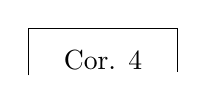
\begin{tikzpicture}\node at (0,0) {\uline{Cor. 4}};\draw (-0.95,-0.2)--(-0.95,0.4)--(0.95,0.4)--(0.95,-0.15);\end{tikzpicture}
\deleted{\unsure{Pour qu'un} \unsure{triplet} $(W,C,F)$ \unsure{soit} \unsure{un} \unsure{triplet}, de Quillen clos, il faut que \unsure{C clos} \unsure{et} \unsure{F clos}, \unsure{à droite}, $(C,TF\overset{\mathrm{def}}=\unsure{C_*})$ et $(TC\overset{\mathrm{def}}=C\cap W\unsure{)|,}$}
\inserted{\unsure{Soit} $W$ \unsure{un loc.} \unsure{mult.} \unsure{non multipli.|non vide|saturé},}
et $(C,TF),(TC,F)$ deux \unsure{précouples} de Quillen tels que $\unsure{TC|TE}\subset C\cap W$, $TF\subset F\cap W$, les cond. suivantes sont équiv.
\[
\begin{aligned}
\text{a)}\quad TC&=C\cap W\\
\text{b)}\quad TF&=F\cap W\\
\text{c)}\quad W&=TF\circ TC\\
\text{d)}\quad &(W,C,\unsure{P|F})\ \text{est un \unsure{triplet|couple}}\\
&\text{de Quillen clos.}
\end{aligned}
\]
}
% archive sheet number: 161
